
\chapter{数学中的意义与形式}

就是这篇《二部创意曲》启发了我,使我构想出本书对话中那两个角色。就像刘易斯·卡罗尔信手借来芝诺的乌龟和阿基里斯一样,我也信手借来刘易斯·卡罗尔的乌龟和阿基里斯。在卡罗尔的对话中,同样的事件一次又一次地发生,只是每一次都发生在更高的层次上,它与巴赫的“无穷升高的卡农”绝妙地相似。即便不谈其中的妙语,卡罗尔的对话也仍然包含有深刻的哲学问题,即:文字和思维是否遵循形式规则?这个问题也是本书的问题。

在本章与下一章中,我们将研究一些新的形式系统。这将使我们对形式系统这一概念有一个更为广阔的视野。读完这两章之后,对于形式系统的力量,以及为什么它们引起了数学家和逻辑学家的兴趣,读者就会有一个相当清楚的认识了。

\section{pq系统}

本章中的形式系统叫做"pq"系统。它对于数学家和逻辑学家并不重要——事实上,它只是我的一个简单发明。它的重要性,实际上仅在于它为在本书中起着相当重要作用的许多概念提供了一个非常好的例子。"pq"系统有三个不同的符号:
\[
  "p" \qquad "q" \qquad -
\]
——字母"p"、"q"和短杠。

pq系统有无穷多条公理。由于不能把它们全部写出来,我们只能用另外的方法描述它们。实际上我们不仅需要对于公理的描述,我们还需要一种辨别某个给出的符号串是否是一条公理的方法。对于公理仅仅做一个描述也许能充分地刻划它们,但是这种刻划是很弱的——与"WJU"系统中对于定理的刻划所存在的问题是一样的。我们并不想仅仅为确定某个符号串是否是公理而花费一段不知多长的——甚至可能是无限长的——时间。所以,我们将给公理这样下定义,使得对于由"p"、"q"和短杠所组成的符号串是否是一条公理,有一个明显的判定过程。

\begin{thm}{定义}
只要$x$仅由一串短杠组成,那么$x-"q"x"p"-$就是一条公理。
\end{thm}
请注意“$x$”在两次出现时必须是代表同一串短杠。比如:$---"q"--"p"-$是一条公理。当然“$x-"q"x"p"-$”这个表达式本身并不是一条公理(因为“$x$”不属于"pq"系统)。它更像是一个铸出所有公理的模子——它被称做公理模式。

"pq"系统只有一条生成规则:

\begin{thm}{规则}
假设$x$、$y$和$z$都代表只包含短杠的特定的符号串,并且假设$x"q"y"p"z$是一条已知的定理,那么$x-"q"y"p"z-$就是一条定理。
\end{thm}
比如让$x$是“$-$”,$y$是“$--$”,$z$是“$---$”,这条规则就是:

\begin{block}
如果$-"q"--"p"---$是一条定理,则$--"q"--"p"----$也是一条定理。
\end{block}
正像生成规则通常的形式那样,这个陈述在一个符号串是否是定理与另一个符号串是否是定理这两者之间建立了因果关系,但并不断定这些符号串本身是否是定理。

对于读者最有用的练习就是为"pq"系统的定理找出一个判定过程。这并不困难,找一会儿就能找出来。不妨试一试。

\section{判定过程}

我假定读者已经试过了。首先我想指出——这也许是太显而易见而不必提起的——\ "pq"系统中的每一条定理都有三组分离的短杠,并且起分离作用的成分依次为"q","p"(这可以由基于“继承性”的一个论证来证明,就是证明"WJU"系统中的定理都是以"W"开头的那种方法)。这就是说,仅仅从形式上,我们就可以排除像
\[
--------"q"--"p"--"p"--"p"--
\]
这样的符号串,指出它不是一条定理。

强调“仅仅从形式上”这几个字似乎显得是笨拙了:除了形式,一个符号串还有什么?有什么其它的东西可能在确定它的性质时起作用?很显然,没有。但是在继续讨论形式系统时,请把这一点记在心里:“形式”的概念会变得更复杂、更抽象。所以我们恐怕得多想一下“形式”这个词的意义。不管情况怎么样,让我们把任何一个以一组短杠开头,然后有一个"q",接着是第二组短杠,然后是"p",最后是另一组短杠这样的符号串都叫作“构形良好的”(简称“良构”)符号串。

让我们回到判定过程上来。是否是定理的标准,是后两组短杠加起来是否等于第一组短杠。例如:$----"q"--"p"--$是一条定理,因为$4$等于$2$加$2$,而$-"q"--"p"--$不是一条定理,因为$1$不等于$2$加$2$。要知道为什么这是正确的标准,首先要看一下公理模式。显然,它只制造满足这个加法标准的公理。其次再看产生规则。假如第一个符号串满足加法标准,那么第二个一定也满足——反之亦然:假如第一个符号串不满足加法标准,则第二个符号串也不满足。这条规则使加法标准成了定理的一个遗传特性:任何一条定理都把这个特性传给由它产生的定理。这就证明了为什么加法标准是正确的。

顺便提一下,我们有一个关于"pq"系统的事实,这一事实使我们可以有把握地说"pq"系统有一个判定过程,甚至在找到加法标准之前就可以这么说。这个事实是:"pq"系统没有因为加长规则和缩短规则这两种相反的力量而复杂化。它只有加长规则。对于任何一个只告诉我们如何从较短的定理得到较长的定理,而永远不会反过来的形式系统,其定理都有一个判定过程。比如,假定给了一个符号串,首先,检查它是不是一条公理(我假设有一个判定公理的判定过程——否则一切就都没有希望了)。如果它是一条公理,那么它也可以称作是一条定理,这个测试就完毕。于是再假定它不是一条公理,那么,它要是一条定理,就一定是从一个较短的符号串得出来的。在逐条地试用各条规则时,不仅能准确地找出可能产生那个符号串的规则,而且还能准确地找出哪一个较短的符号串会是“家谱”中它的上一代。用这种方法,把问题“归约”成为去确定几个新的、但是较短的符号串是否都是定理,然后对它们依次地进行同样的测试。可能出现的最坏情形是产生出大量的、越来越多的、但是越来越短的需要测试的符号串。当以这种方式一步一步地回溯时,就一定会距离一切定理的源泉——公理模式越来越近。越来越短不会是无限的,因此,最终或是发现那些短符号串的其中一个是一条公理,或是到达了某一个无法再往回退的点——也就是没有一个短符号串是公理,并且没有一个短符号串可以通过某条规则或其它倒退步骤进一步缩短。这表明了在形式系统中,只有加长的规则确实是没有多大意思的。是加长与缩短的规则交互作用使形式系统具有了某种魅力。

\section{自底向上之别于自顶向下}

上述方法可以称为自顶向下的判定过程,相比之下,现在要给出的判定过程可以称为自底向上。它使人想起那个怪物用来在WJU系统中系统地生成定理的方法。但是,由于有公理模式,现在的情形要复杂些。我们将准备一只桶,当定理生成了以后,我们就把它们丢进桶里。以下便是具体做法:
\begin{description}[labelwidth=2\ccwd, labelsep=0pt,
  align=fillright, leftmargin=4\ccwd]
\item[(1a)]将最为简单的公理($--"q"-"p"-$)丢进桶里。
\item[(1b)]对于桶里的每个公理应用推理规则,将推得的结果丢进桶里。
\item[(2a)]将第二简单的公理丢进桶里。
\item[(2b)]对桶里的每个符号串应用规则,并将结果都丢进桶里。
\item[(3a)]将第三简单的公理丢入桶里。
\item[(3b)]对桶里的每个符号串应用规则,并将结果都丢进桶里。
\item[]等等,等等
\end{description}

略微想一想之后,可以看到,你用这种方法可以把"pq"系统里的每一条定理都产生出来。同时,随着时间的延续,桶里会装入越来越长的定理。这又是由于没有缩短规则的结果。因此,假如你有一个特定的,像$-----"q"-"p"---$这样的符号串,并且想测试一下它是不是一条定理,只要按照上述标了号码的步骤,一直不断地检查是否出现了这个符号串。如果它出现了——它就是定理。假如到了某一个时候,放进桶里的每个东西都比要测试的这个符号串长,那么,就可以丢开它——它不是一条定理。这个判定过程是自底向上的,因为它是从基础,也就是说是从公理开始往上进行的。前面的那个判定过程是自顶向下的,因为它恰恰与此相反:它是向着基础往回进行的。

\section{同构产生意义}

现在我们涉及到了本章——实际上是本书的——中心问题。也许读者已经想到,"pq"定理很像是加法。$-----"q"--"p"---$这个符号串是一条定理,因为5等于2加3。读者甚至可以认为$-----"q"--"p"---$这条定理是一个用奇怪的记法记下来的陈述,它的意义是$5$等于$2$加$3$。这样看问题合乎道理吗?嗯,我是有意地选择“"q"”,因为英语里“等于”这个词是equal,而选择“"p"”是因为英语里“加”这个词是plus。那么,$-----"q"--"p"---$这个符号串真的意味着“$5$等于$2$加$3$”吗?

是什么东西使我们那样想的呢?我的回答是:我们在"pq"定理与加法之间看到了同构。在导言中,“同构”这个词的定义是保存信息的变换。现在我们可以深入到那个概念中去,从另一个角度看一看。“同构”这个词的适用情景是:两个复杂结构可以互相映射,并且每一个结构的每一部分在另一个结构中都有一个相应的部分。这里“相应”的意思是:在各自的结构中,相应的两个部分起着相类似的作用。“同构”这个词的这种用法是从数学中一个更精确的概念那里得来的。

当一个数学家发现在他所知道的两个结构之间有同构关系时,就会感到很愉快。这种关系常常“从天而降”,让人惊喜不已。认识到两个已知结构有同构关系,这是知识的一个重要发展——并且我认为,正是这种对于同构的认识在人们的头脑中创造了意义。关于对同构的认识要说的最后一点是:形象地说,由于它们可以是各种各样千姿百态的,人们并非总能搞清何时才是真正地发现了同构。因此,“同构”具有通常的词所具有的模糊性。这一点是它的缺陷,但也是长处。

对于这种情况,我们有一个关于同构概念的极好范例。我们的同构有一个“较低的层次”——也就是,在两个结构中各个部分之间的映射关系:
\[
\begin{array}{r>{\iff}cl}
  "p" & & \text{等于} \\
  "q" & & \text{加}\\
    - & & 1 \\
   -- & & 2 \\
  --- & & 3 \\
      & \multicolumn1c{\text{等等}}
\end{array}
\]
这种符号与词之间的对应关系有一个名称:解释。

其次,在一个高一点的层次上,真陈述(也称“真理”)和定理之间存在着对应。但是,请注意,如果不在事先给这些符号选定一种解释,这种高一层次的对应是看不出来的。因此,更准确地说,对应是存在于真陈述和经过解释的定理之间的。不管怎么说,我们是展现了一个两层的对应,这在所有的同构中是典型的。

当遇到一个你一无所知的形式系统,并且假如你希望去发现它某种隐藏的含义时,你的问题就在于如何给它的符号赋予一种有意义的解释——也就是,通过某种方式,使得在真陈述和定理之间出现一个高层次的对应。在找到一组联系于这些符号的合适的词之前,你可能要在黑暗里进行一番摸索。这与破译密码或者释读用一种失传了的文字写成的铭文(比如克里特岛的线形文字B)非常相似。释读的唯一方法就是建立在以知识为基础的猜想上的试错法。当你发现一个好的选择,一个“有意义”的选择时,突然间就觉得顺当了,并且工作的速度大大加快了。不久,件件事情就都各就各位了。约翰·查德威克的《克里特岛线形文字的释读》一书中就包含有这种令人激动的经历。

但是,对挖掘一个已经毁灭了的文明时发现的形式系统进行释读,这种机会实在太少了。数学家(近来还有语言学家、哲学家和其它人)是仅有的使用形式系统的人。而且他们心里对于他们所使用和出版的形式系统总是有个解释的。这些人的想法是:建立一个形式系统,它的定理同构地反映一部分现实世界。在这种情况下,对于符号的选择是有高度目的性的,就像是对于符号串的生成规则的选择那样。我设计"pq"系统时就是这样的。你可以看出来,我为什么选用了我所选的符号。定理与加法同构这一点不是偶然的,同构之所以发生,是因为我有意地找到了一种通过符号形式反映加法的方法。

\section{有意义的解释与无意义的解释}

你可以选择与我不同的解释。你无需使每条定理都成为真的。但要是建立一个解释,使每条定理都成为假的,这也没什么意思。当然,要是作一个解释,其中的定理和真理之间没有一点正的或反的相关性,这就更没有意思了。因此,让我们区别开对于形式系统的两类解释。首先,我们可以有一些无意义的解释,在这种解释下,看不到系统中的定理与现实世界之间有什么同构关系。这样的解释多得很——任何随意的选择,都是这样的解释。例如下面这个:
\[
\begin{array}{r>{\iff}cl}
  "p" & & \text{马}  \\
  "q" & & \text{幸福} \\
  -   & & \text{苹果}
\end{array}
\]

那么$-"q"-"p"--$就获得了一个新的解释:“苹果马苹果幸福苹果苹果”——很有诗意的,它可能会打动马,甚至可能使它们喜欢这种对于"pq"符号串的解释!这种解释没什么“意义”。在这种解释中,定理听起来既不比非定理真一些,也不比它们好些。一匹马可以欣赏“幸福幸福幸福苹果马”(映射成$"ppp"-"q"$),就像它欣赏任何一条经过解释的定理一样。

另一种解释叫做有意义的。在这种解释下,定理和真理是相对应的——也就是,同构存在于定理与现实的某一部分中。这就是区别解释与意义的好处。任何已有的词都可以用来解释“"p"”,但是“加”是我们所碰到的唯一有意义的一个。总的来说,“"p"”的意思看来应该是“加”,虽然它还可以有成千上万个不同的解释。

\section{主动意义之别于被动意义}

如果深一步地理解,这一章的最重要的事实也许是:"pq"系统似乎在迫使我们认识到,形式系统中的符号虽然一开始没有意义,但至少在发现了同构关系时,不可避免地会带上某种“意义”。然而,形式系统中的意义与语言中的意义的区别是非常重要的。这区别是:在语言中,当我们知道了一个记号的意义,我们就能基于这个记号做出新的陈述。从某种意义上说,语言中的意义是“主动的”,因为它为创造句子带来了一条新规则。就是说,我们对于语言的掌握,不像是对于一件完成了的产品那样。当我们知道了新的意义的时候,造句子的规则也增加了。另一方面,在形式系统中,定理都是运用产生式规则事先定义了的,我们可以选择以定理与真陈述之间的同构(假如可以找到的话)为基础的“意义”。但是,不是说这样就准许我们在已建立的定理之外增加新的定理。这就是第一章中形式化要求所警告过的。

在"WJU"系统中,当然没有什么东西诱惑我们去超出那四条规则,因为还没有找到或发现一种解释。但是在这里,在我们的新系统中,人们可能受到新发现的每一个符号的“意义”的影响而认为符号串$--------"q"--"p"--"p"--"p"--$
是一条定理。至少,人们可能希望这个符号串是一条定理。但是愿望并不能改变它并不是一条定理这一事实。仅仅因为$8$等于$2$加$2$加$2$加$2$,就认为它“一定”是一条定理,这是极大的错误。甚至赋予它意义就是错误的,因为它不是良构的,而我们的有意义的解释整个都是从良构符号串中得出的。

在一个形式系统中,意义一定是“被动的”。我们可以根据其组成符号的意义来读每个符号串,但是我们没有权力只根据我们给符号指定的意义而创造出新的定理。经过解释的形式系统是横跨在没有意义的系统与有意义的系统之间的。可以认为,它们的符号串是“表达”事物的,但这也必定是系统的形式性质的产物。

\section{双重意义!}

现在我要破除一种错觉,即认为已经找到了pq系统中符号的唯一意义。考虑下列联想:
\[
\begin{array}{r>{\iff}cl}
  "p" & & \text{等于} \\
  "q" & & \text{加}\\
    - & & 1 \\
   -- & & 2 \\
      & \multicolumn1c{\text{等等}}
\end{array}
\]
那么$-----"q"--"p"---$就有了一个新的解释:“$5$减$2$等于$3$”。当然这是一个真陈述。在这种新的解释之下,所有的定理都将是真理。这就像原来那个解释一样有意义。很显然,“哪一个是这个符号串的唯一意义?”就成了一个很愚蠢的问题。解释只要精确地反映现实世界的某种同构,就是有意义的。当现实世界中的不同方面彼此同构时(这里是说加法和减法),一个形式系统可以与这两者都同构,因此可以有两种被动意义。这种符号和符号串的二值性是一个极其重要的现象。在这里,它似乎是不足道的、奇怪的、令人恼火的。但是,在以后更深入的讨论中,它还会再次出现,并带来极丰富的内容。

现在来把我们对于"pq"系统所做的观察作一个总结。给定两个有意义的解释,那么用其中的任何一个,每个良构的符号串都对应于一个合法的断言——有些是真的,有些是假的。在一个形式系统中,良构符号串的含义就是:当对它一个符号一个符号地去解释时,就产生合语法的句子(当然,这取决于如何解释。但是,通常在人们脑子里有一种解释)。定理出现在良构符号串中。这些定理是由一个公理模式和一条生成规则来定义的。我发明"pq"系统的目的是要模仿加法:我想让每一条定理在解释之下都表达一个真正的加法;反之,我想让每一个真正的恰好是两个整数相加的加法都能翻译成一个是定理的符号串。我的目的达到了。请注意,这样,所有的错的加法,像“$6$等于$2$加$3$”,将映射成一些不是定理的良构符号串。

\section{形式系统和现实}

在那些基于现实的一部分的形式系统中,"pq"系统是我们遇到的第一个实例,并且看起来模仿得很好。在这种模仿中,它的定理和有关那部分现实中的真理同构。然而,现实和形式系统是互相独立的,并不需要意识到在两者之间存在着同构关系。每一方面都独立存在——不论我们知道不知道$2$等于$1$加$1$,$--"q"-"p"-$都是一条定理;并且不论我们是否把它与加法相联系,$--"q"-"p"-$总是一条定理。

读者可能想知道,构造这样或者那样的形式系统,是否能就其论域(它的解释所在的领域)中的真理给我们一些启发。通过构造pq定理,我们知道了什么新的加法吗?当然没有,但是我们知道了关于加法作为一种操作的性质——也就是说,它很容易用支配无意义符号的印刷符号(以下简称印符)规则加以模仿。这仍然不应使人惊异,因为加法是那么一个简单的概念。加法可以很简单地体现在一部机器的旋转的齿轮之中,就像在现金出纳机中那样。

但是很清楚,就形式系统而言,我们几乎只触及了表面。人们很自然地想知道,现实的哪一部分能够用一组支配无意义符号的形式规则来加以模仿。现实世界的一切都可以变为形式系统吗?从一个很广的意义上说,回答可能是肯定的。比如,人们可以设想,现实世界本身只不过是一个非常复杂的形式系统。它的符号不是在纸上移动,而是在一个三维空间里运动,它们是组成一切事物的基本粒子(这里包含着一个隐含的假定,即:物质的可分性是有尽头的,因此,基本粒子这个词是有意义的)。“印符规则”是物理法则,它告诉人们如何根据给定的时刻从给出的所有粒子的位置和速度,得出属于“下一个”瞬间的一组新的位置和速度。所以这个宏伟的形式系统的定理,就是粒子在宇宙历史中不同时间的可能布局。唯一的公理是所有粒子在“时间的开始”时的原始布局。这是一个非常宏伟的设想,然而它只有纯粹的理论意义。另外,量子力学(及物理学的其它部分)也使人们对于上述概念所含的理论价值产生了某种怀疑。从根本上说,我们是在问宇宙是否是以完全确定的方式运动,而这是个尚未解决的问题。

\section{数学与符号处理}

我们将不去讨论那么大的一幅图景,而只以数学做为我们的“现实世界”。这里出现了一个严重的问题:假如我们试着按照某数学分支构造一个形式系统,我们如何确定我们是否已把这项工作做得很准确了呢?尤其是假如我们不是已经百分之百地熟悉了那部分数学的话。假定形式系统的目的是要给我们带来那个学科的新知识。那么,在我们证明了同构是完全的之前,怎么知道对于每一条定理的解释都是真理?并且,如果我们在开始时不知道那个学科中的所有真理,我们又怎样证明同构是完全的呢?

假定在某个遗址的发掘中,我们确实发现了某种神秘的形式系统。我们可以试验各种不同的解释方法,并且也许最终碰上了一种看起来使每一个定理成为真理,每一个非定理成为“假理”的解释。但这是一种只能在有穷多个情形里进行直接检验的东西,而定理的集合多半可能是无穷的。我们怎么会知道所有的定理在这种解释方法之下表达了真理?除非我们知道关于形式系统及相应论域的每一个细节。

当我们企图将自然数世界(也就是非负整数:$0$, $1$, $2$, $3$,\ldots)和一个形式系统的印刷符号相匹配时,我们就会发现自己是处于这样一种奇怪的境地了。我们将努力去理解,我们在数论中称作“真理”的,和我们借符号处理所能做到的,这两者之间是什么关系。

因此,让我们简略地看看,当我们称数论中的某些陈述为真,而另一些为假时,其根据是什么。$12$乘以$12$得多少?人人皆知,得144。但是有多少给出这个答案的人在他们的生活中曾经画过一个$12\times 12$的长方形,然后数它的小方格?多数人认为画格和数它们是不必要的。他们会代之以在纸上写下如下的式子作为证明:
\[
  \opmul[displayintermediary=all]{12}{12}
\]
这就是“证明”了。几乎所有的人都相信,如果去数小方格,一定是$144$个,几乎没有人会对此得数感到怀疑。

当考虑确定$987654321\times 123456789$的值时,这两种观点的差别就会看得更清楚了。首先,根本不可能构造一个合适的长方形;更糟糕的是,即便造出来了,也得要大批的人用几个世纪的时间,不停地数那些格子。而只有极易轻信的人,才愿意相信他们最后数出的结果。某个人、在某个地方、以某种方式出个小小的失误,这简直是太可能发生的事了。因此,究竟是否有可能知道它的得数?如果信任按照某种简单规则处理数字的符号操作过程,回答是肯定的。这个过程作为一种得到正确答案的方法提供给孩子们,而对于许多孩子来说,这个过程的道理由于在这么多的符号中摆弄来摆弄去,往往就显得不清楚了。乘法的数字变换法则多半是基于加法、乘法的少数几条性质,而这些性质被假定是对于所有的数都有效的。

\section{算术的基本法则}

对我所说的那种假定,现在就可以说明如下。设划了几个道道:
\begin{center}
/\quad //\quad //\quad //\quad /\quad /
\end{center}
现在数一数它们。同时另外一个人从另一头数。两个人会得到同一个答案,这一点是否清楚?数的结果与计数的方法是无关的。这就是对于什么是计数的一种假定。要试图证明这一点将是毫无意义的,因为它太基本了,不管是看得出来还是看不出来。如果看不出来,就是证明也不会有一点儿帮助。

从这样的假定中,可以得出加法的交换律和结合律(也就是说:第一:永远有$b+c=c+b$,第二:永远有$b+(c+d)=(b+c)+d$)。同样的假定也可以引出乘法交换律和结合律,这只要想想许多小方块汇集在一起形成一个大的长方体的情形。乘法的交换律和结合律就是这样一种假定:以各种方式旋转那个长方体时,小立方体的数量不会改变。这些假定不是在所有可能的情况下都可以验证的,因为,这类的情况是无穷的。我们认为这是当然的,我们像相信其它事物一样深信它们(假如我们想到它们)。我们从街上走过时,口袋里的钱上上下下地相撞,但是数量不会改变。如果我们把我们的书装入盒子中,放进汽车,开一百里,把盒子拿下汽车,打开,把书放上一个新的书架,书的数量也不会改变。所有这些都是数的性质的一部分。

有这样的人,当某种不可否认的事实一旦写下来时,总是喜欢找点理由,使那个“事实”干脆成了假的。我就是这样的人。在我刚刚写下上面的关于线段、钱和书等例子的时候,我就又设想了一些情境,在其中它们可能并不成立。读者也可以这样做。它说明抽象的数与日常生活中我们使用的数确实是很不相同的。

人们喜欢造些违反基本算术的说法,以便说明某种“更深刻的”真理。比如“$1+1=1$”(对恋人而言),或者“$1+1+1=1$”(三位一体)。很容易从上述说法里找出漏洞,比如,指出在上述两种情况中,为什么使用加号是不合适的。但这样的情况多得很。两滴雨水从窗户玻璃上流下来合成了一滴,$1$加$1$是不是等于$1$?一朵云彩分成两朵——还要更多类似的证据吗?发生的事情可以称作“加”,或者需要别的什么词,在这两者之间划一条明显的界限可不是轻而易举的。如果你考虑这个问题,你大概就会提出关于空间中物体的分隔之类的标准,并且肯定每一种物体与其它物体有很明显的区别。但是如何去数思想呢?如何去数组成大气的气体的数量?假如查一查的话,大概能在某个地方发现一个像“印度有十七种语言和四百六十二种方言”这样的陈述。这样精确的陈述倒多少令人感到奇怪了,因为“语言”和“方言”这两个概念本身就是模糊的。

\section{理想的数}

数作为一种“实在”是不守规矩的。然而,人们有一种古老的内在感觉,即数不应该不守规矩。在数的抽象概念中,就有那么一种纯净的东西,独立于数念珠、方言或云朵。应该有一种谈论数的方式,这种方式不会总是受到现实所具有的那种糟糕状况的侵入和捣乱。支配“理想”数的铁定的规则构成了算术,并且进一步构成了数论。在把作为实际事物的数转变成作为形式事物的数的时候,只有一个有关的问题需要提出来。一旦你决定了要把所有数论装入一个理想的系统,是否真有可能彻底地做到这一点呢?数是否那么整洁,那么有规律,像结晶一样,以至于形式系统的规则能彻底地把握它们的性质?艾舍尔最漂亮的画之一《释放》(\fig{13}),就是形式与非形式之间的绝妙的对比,它还有一个迷人的过渡区域。数真的像鸟那么自由吗?它们被囚禁在遵守规则的系统中时,也像那些鸟一样难以忍受吗?现实中的数与写在纸上的数之间是否有一个不可思议的过渡区域?

\begin{figure}
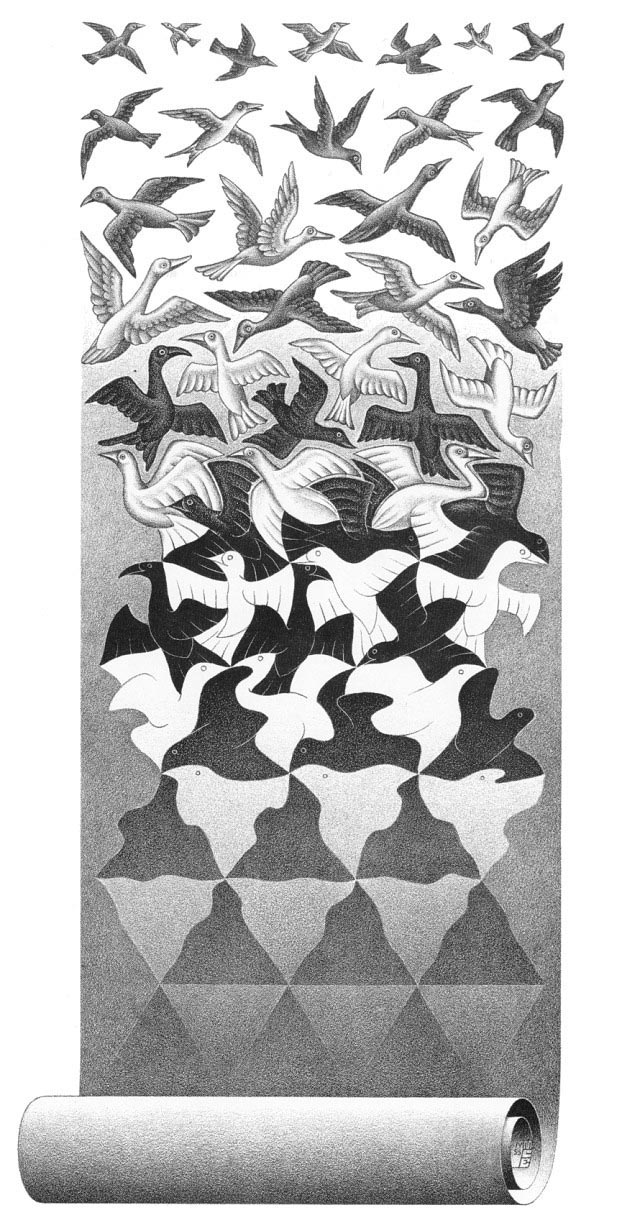
\includegraphics[height=.9\textheight]{img_013.jpg}
\caption[释放,艾舍尔作。]
  {释放,艾舍尔作(石版画,1955)。}
\end{figure}

说到自然数的性质时,我不是单指像“特定的两个整数的和”这样的性质。这种性质可以通过计数找出来。每一个在二十世纪里长大的人都不会怀疑像这样的计数以及加法、乘法等等这些过程的可机械化性。我所指的性质是数学家有兴致去探讨的那些问题,而计数过程不足以为那些问题提供答案——甚至在理论上,也不足以提供答案。让我们举一个古老的关于自然数性质的例子:“有无穷多个素数。”首先,没有一个计数过程能够证实或推翻这一断言。我们可以做到的,最多只不过是数上一会儿有多少个素数,然后承认,确实“有不少”。但是,不管你数出了多少素数,你的结果都无法确定素数的个数是有穷的还是无穷的。总是数不完。这个陈述——被称做“\emph{欧几里德定理}”(请注意是黑体字)——不是显然的。看上去它可能是合理的和令人信服的,但不是显然的。然而,欧几里德及后来的数学家一直说它是真的。什么原因呢?

\section{欧几里德的证明}

原因是,推理告诉他们是这样的。让我们来看看这种推理。我们来看一个欧几里德证明的变种。这个证明告诉人们,不论挑出哪一个数,都还有一个比它大的素数。挑出一个数——$N$,把所有从$1$到$N$的正整数相乘,换句话说,也就是做N的阶乘,写作“$N!$”。得到的数可以被从$1$到$N$之间的任何数除尽。然后在$N!$上加上$1$,结果这个数就
\begin{itemize}
\item 不能是$2$的倍数(因为当被$2$除时,余$1$);
\item 不能是$3$的倍数(因为当被$3$除时,余$1$);
\item 不能是$4$的倍数(因为当被$4$除时,余$1$);
\item ……
\item 不能是$N$的倍数(因为当被$N$除时,余$1$);
\end{itemize}
换句话说,假如$N!+1$是可以被除尽的(除了被$1$和它本身除之外),也只能是被比$N$大的数除尽。因此,或者它本身是素数,或者它的素因数比$N$大。但是不论是哪种情况,我们已经表明,都一定有比$N$大的素数存在。不论$N$是什么数,这个论证过程都能进行。因此,不管$N$是什么数,都有一个素数大于$N$。至此,就完成了素数有无穷多个这一证明。

顺便说一下,这最后一步叫做推广。在今后更形式化的上下文中,我们还会遇到它。在那里我们就单独一个数($N$)来进行一个论证,然后指出我们用的$N$是非特定的,因此我们的论证是一般性的。

欧几里德的证明是典型的所谓“真正的数学”。它简洁、优美且令人信服。它表明人们可以通过一些很简短的步骤从起点走出很远。在我们这个例子里,起点是关于乘法和除法等等的基本概念。短小的步骤是指推理的步骤。虽然每一个单个的推理步骤看起来是显然的,但最后的结果并不显然。我们永远不能直接地检查这个陈述是否是真的,然而我们相信它,因为我们相信推理。如果你接受推理,似乎就别无选择。一旦你同意听欧几里德把话讲完,你就得同意他的结论。这是件幸事——因为这意味着数学家对于把什么样的陈述标为“真的”,把什么样的标为“假的”,永远持一致意见。

这个证明是有条理的思维过程的一个例子。每一个陈述都以一种不可抗拒的方式与前一个陈述有着联系。这就是为什么称它为“证明”而不只是“好的证据”。在数学中,目的总是给予某个不那么显然的陈述一个滴水不漏的证明。存在有这种以滴水不漏的方式联系在一起的步骤,这一事实本身就暗示着可能存在一个具有模式的结构把这些陈述联在一起了。展示这个结构的最好办法是找一些新的词汇——有特定的风格、由符号构成的词汇——仅适于表达关于数的陈述的新词汇。然后,我们可以看看经这些新词汇翻译后的证明。它将是一行接一行地以某种可以检查的方式联系在一起的一些陈述。但是,因为这些陈述是由具有特定风格的小符号集合来表示的,所以它们具有模式的样子。换句话说,虽然大声朗读出来时它们好像是关于数以及它们的性质的陈述,但当把它们写在纸上时,它们仍然好像是抽象的模式——并且这个证明的一行接一行的结构可能开始变得像是模式按照某些印符规则在缓慢地变换。

\section{绕过无穷}

虽然欧几里德的证明是一个关于所有的数都有某种性质的证明,它却回避了分别讨论无穷多种情况中的每一个。它用像“不管是什么”或者“不论$N$是一个什么数”这样的话来绕过它。我们也可以使用“所有的$N$”这样的词再陈述一遍这个证明。知道了合适的上下文及使用这些词语的正确方式,我们就永远不需要处理无穷多个陈述。我们只要处理两三个概念,比如“所有”这个词——虽然它本身是有穷的,但它体现了无穷。通过使用它们,我们避开了要证明无穷多个事实这种表面问题。

我们使用“所有”这个词的可能方式是由推理的思维过程来规定的。也就是说,在我们使用“所有”这个词时,要遵循一些规则。我们也许没有意识到它们,并且倾向于认为,我们是在这个词的意义的基础上操作的。但是,这毕竟只是一种迂回的说法,实际上我们是由一些从未摆出来的规则所指引的。我们一生中总是在某些句型中使用某些词,但我们不把这些句型叫做“规则”,而是把我们的思维运转过程归因于词汇的“意义”。这个发现在通向数论形式化的漫长道路上是一个关键性的认识。

假如我们越来越仔细地研究欧几里德的证明,我们就会看到,它是由许许多多小的——几乎是无穷小的——步骤组成的。假如把所有这些步骤都一行一行地都写出来,这个证明会难以置信地复杂。对于我们的头脑来说,把许多步骤压缩在一起形成单个句子是最为清晰的。假如我们用慢动作来观察这个证明,我们就会开始察觉到一个个的框架。换句话说,这个解剖过程到此为止,这之后我们就遇到推理过程的“原子化”性质。一个证明可以分解成一系列小而不连续的跳跃。但从一个更高更便利的角度来观察它的时候,这些步骤是很平滑地过渡的。在第八章中,我将说明一种把证明分成原子单位的方法,读者会看到它涉及了许多步骤,多得令人难以置信。即使这样,它或许也不应该让你太惊异。当欧几里德发明这个证明时,一定有几百万个神经元(神经细胞)参加了操作,其中有许多仅在一秒钟内就被激活了几百次。仅仅说出一个句子就要涉及成千上万个神经元。假如欧几里德的想法那么复杂的话,说它的证明包含了巨大数目的步骤就有意义了(他脑中神经元的活动与我们的形式系统里的一个证明可能没有什么直接联系。但是两者的复杂程度是可以相比的。这就好像是大自然想要使“素数有无穷多”这个证明的复杂性保持恒定,即使涉及到的系统相互之间极其不同)。

在下面的几章中,我们将构造出一个形式系统:\pnum{1}它包含一个具有特殊风格的词汇表,所有的关于自然数的陈述都可以通过它来表达;\pnum{2}它有与所有看起来必要的推理类型相对应的规则。一个很重要的问题是:我们那时所给出的、用于符号处理的规则,是否真的与我们通常的心理推理能力相等(就数论而言)——或者更一般地说,用某种形式系统来达到我们思维能力的水平,在理论上是否有可能。
